\chapter{Oracle Aplication Express}

\section{Cara Membuat Aplikasi Akademik Sederhana}

\begin{enumerate}





\begin{figure}[!htbp]
\item[1] Pertama, login terlebih dahulu ke oracle Apex Online, lalu klik object browser.
    \begin{center}
    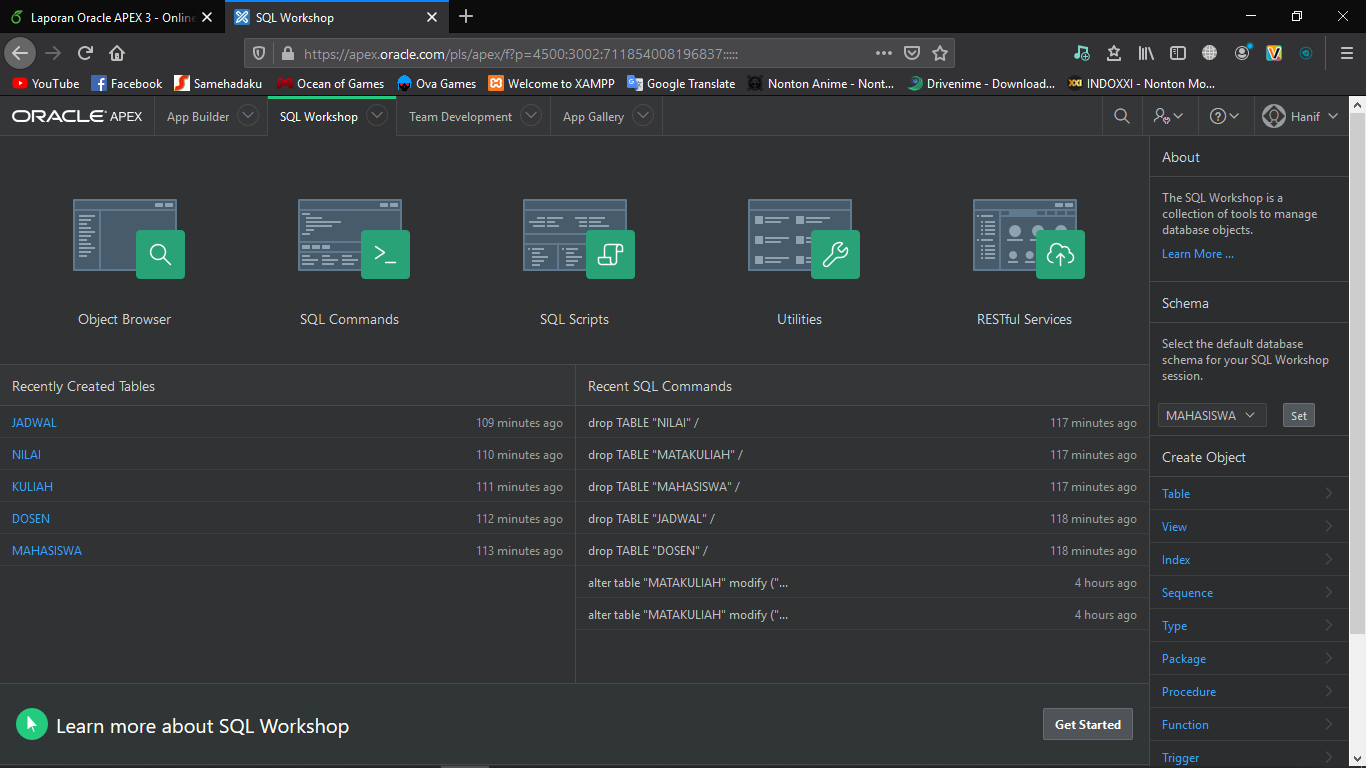
\includegraphics[scale=0.3]{figures/Screenshot(43).png}
    \end{center}
    \end{figure}
    
\begin{figure}[!htbp]
\item[2] Disini saya sudah menggunggah file table dosen, jadwal, kuliah, mahasiswa dan nilai.
\begin{center}
    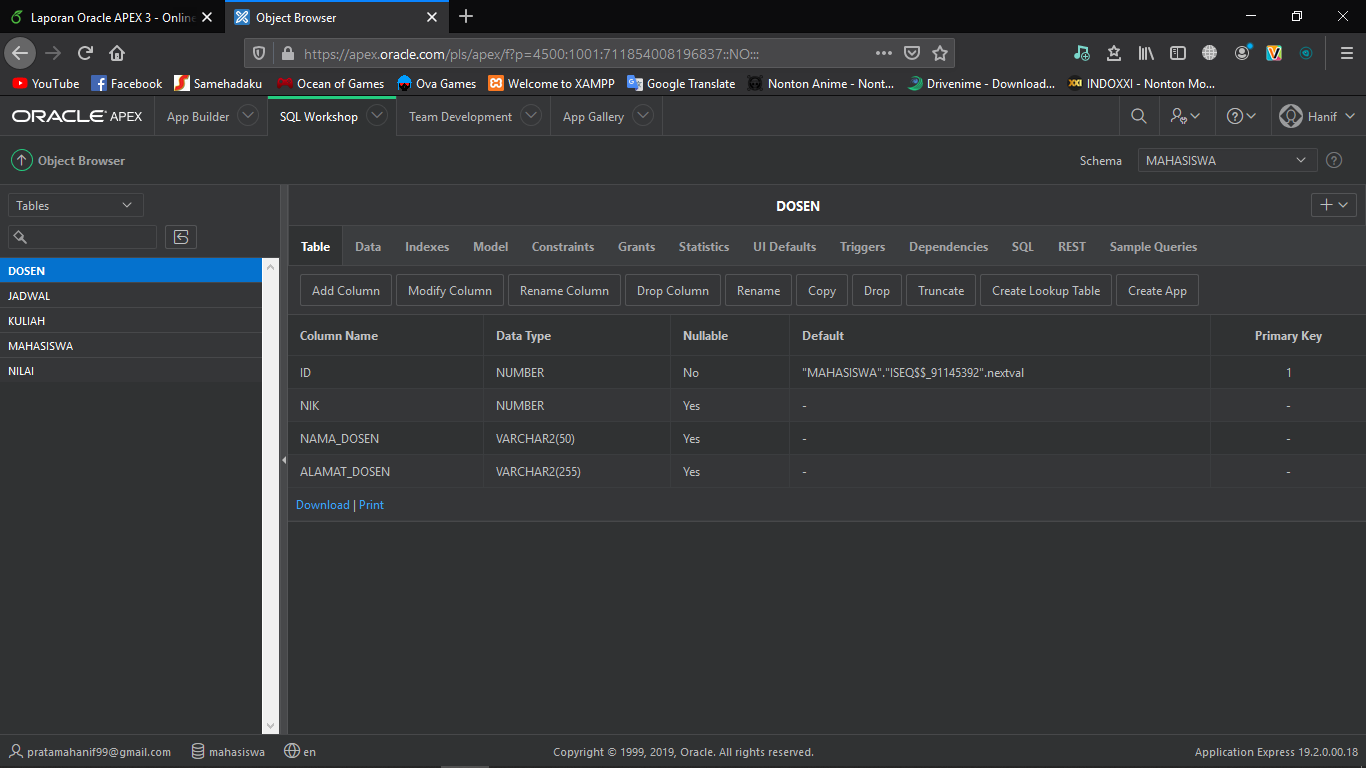
\includegraphics[scale=0.3]{figures/Screenshot(44).png}
    \end{center}
    \end{figure}
    
\begin{figure}[!htbp]    
\item[3] Namun, disini kita harus menghapus kolom ID pada semua tabel karena yang akan dijadikan primary key bukanlah ID. Caranya adalah pilih drop coloum, lalu pilih kolom ID.
\begin{center}
    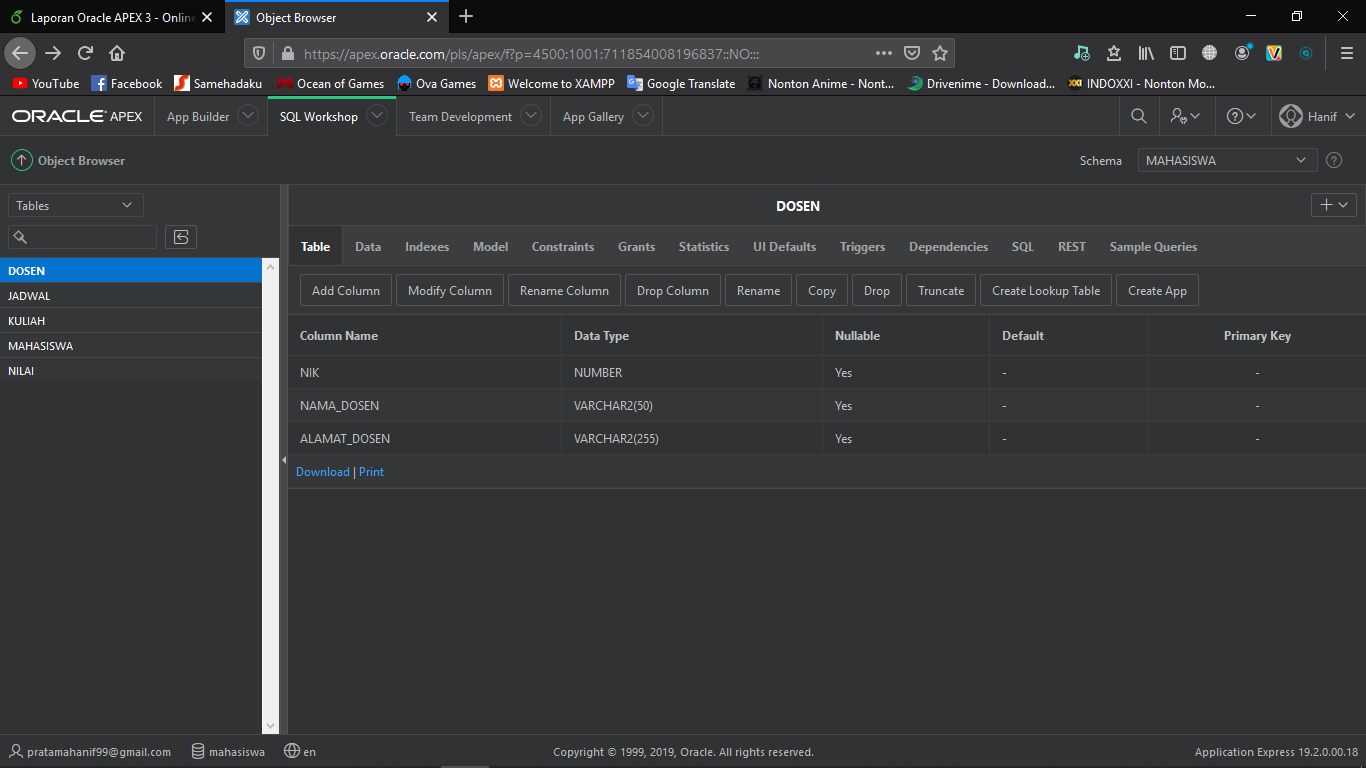
\includegraphics[scale=0.3]{figures/Screenshot(45).png}
    \end{center}
    \end{figure}

\begin{figure}[!htbp]
\item[4] Setelah itu, buat kolom NIK pada tabel dosen, kolom NIM pada tabel mahasiswa dan kolom kode pada tabel kuliah menjadi primary key. Caranya adalah pilih constraint, lalu pilih create, setelah itu pilih primary key dan pilih kolom yang akan dijadikan primary key.
\begin{center}
    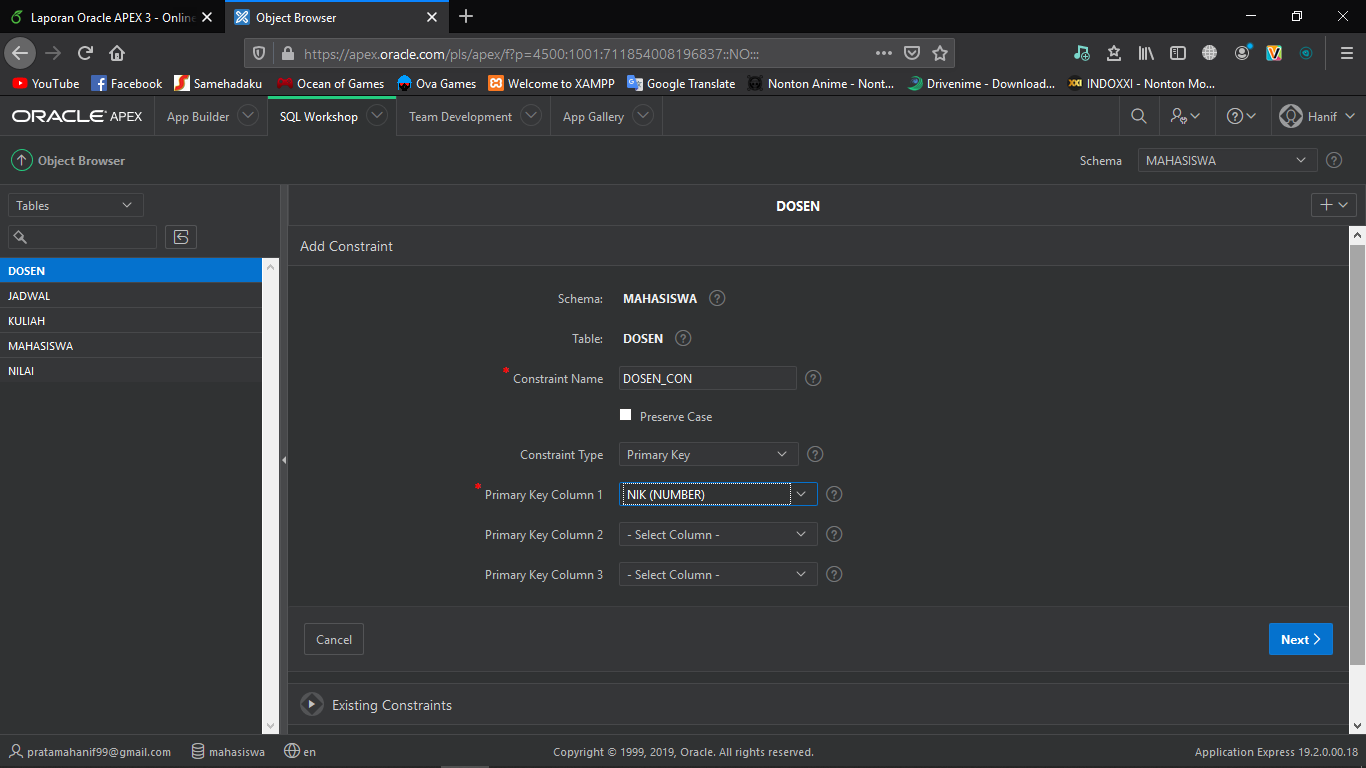
\includegraphics[scale=0.3]{figures/Screenshot(53).png}
    \end{center}
    \end{figure}

\begin{figure}[!htbp]    
\item[5] Buat foreign key di tabel jadwal dan dan nilai. Buat foreign key pada kolom kode dan nik di tabel jadwal. Setelah itu, buat foreign key pada kolom kode dan nim di tabel nilai. Caranya adalah, pilih constraint, lalu pilih create, setelah itu pilih foreign key dan pilih atribut yang ingin dijadikan foreign key, lalu pilih table yang menjadi asal atribut tersebut.  \begin{center}
    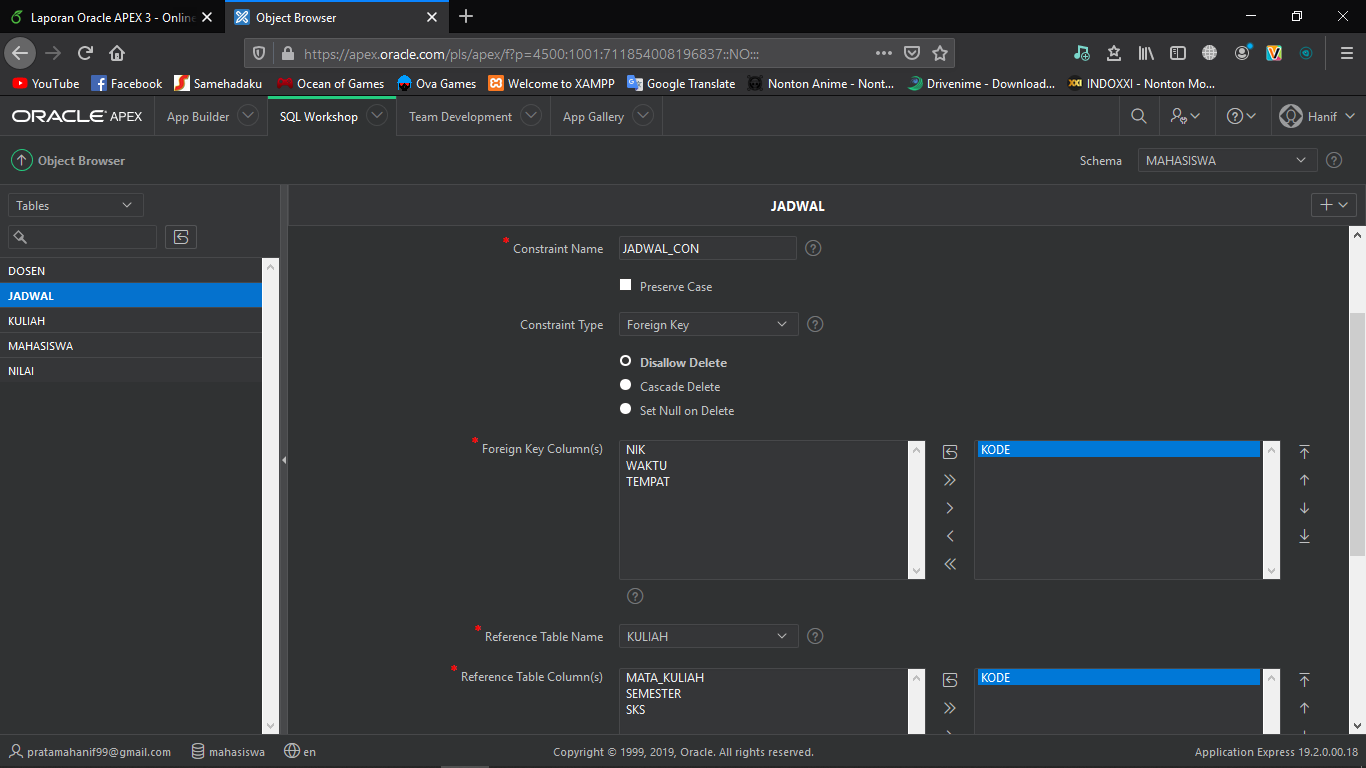
\includegraphics[scale=0.3]{figures/Screenshot(47).png}
    \end{center}
    \end{figure}
    
\begin{figure}[!htbp]
\item[6] Masuk ke App Builder, pilih create.
\begin{center}
    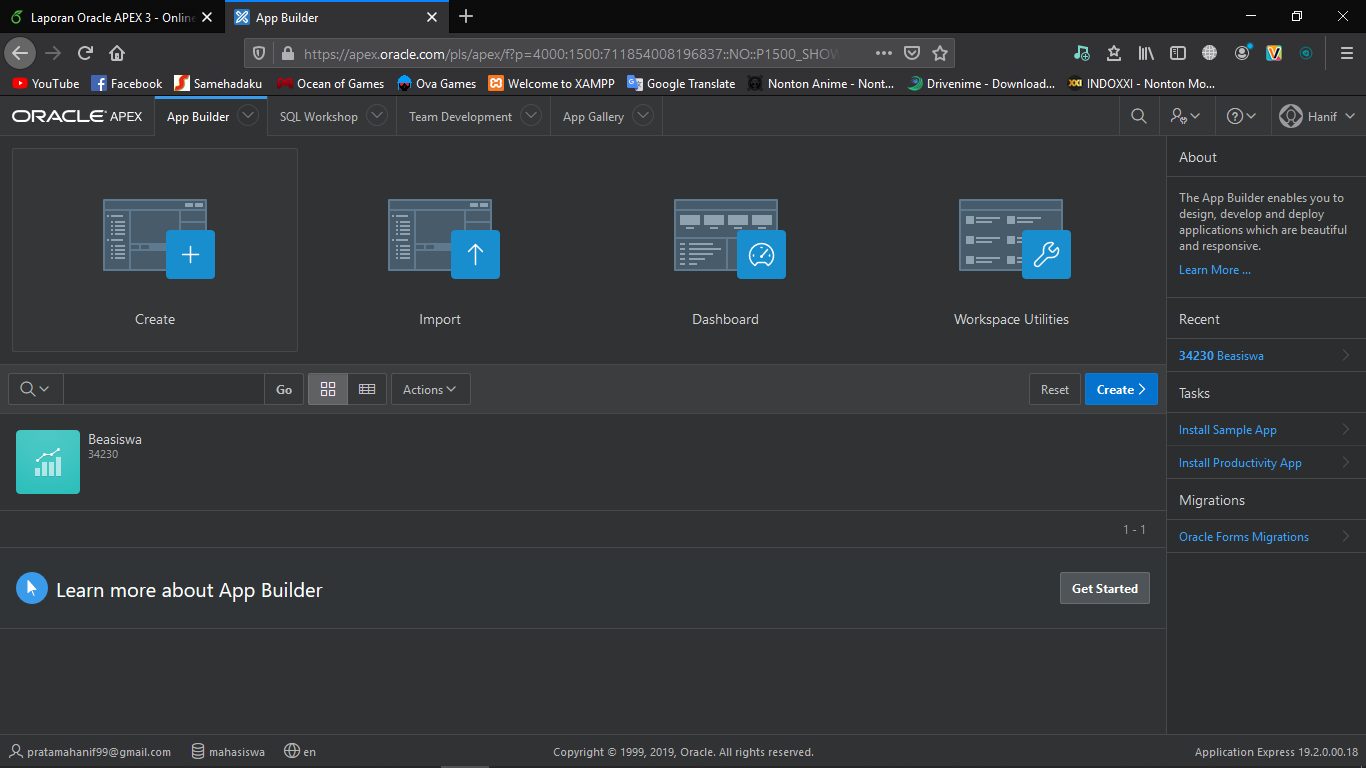
\includegraphics[scale=0.3]{figures/Screenshot(50).png}
    \end{center}
    \end{figure}
    
\begin{figure}[!htbp]    
\item[7] Pilih new application.
\begin{center}
    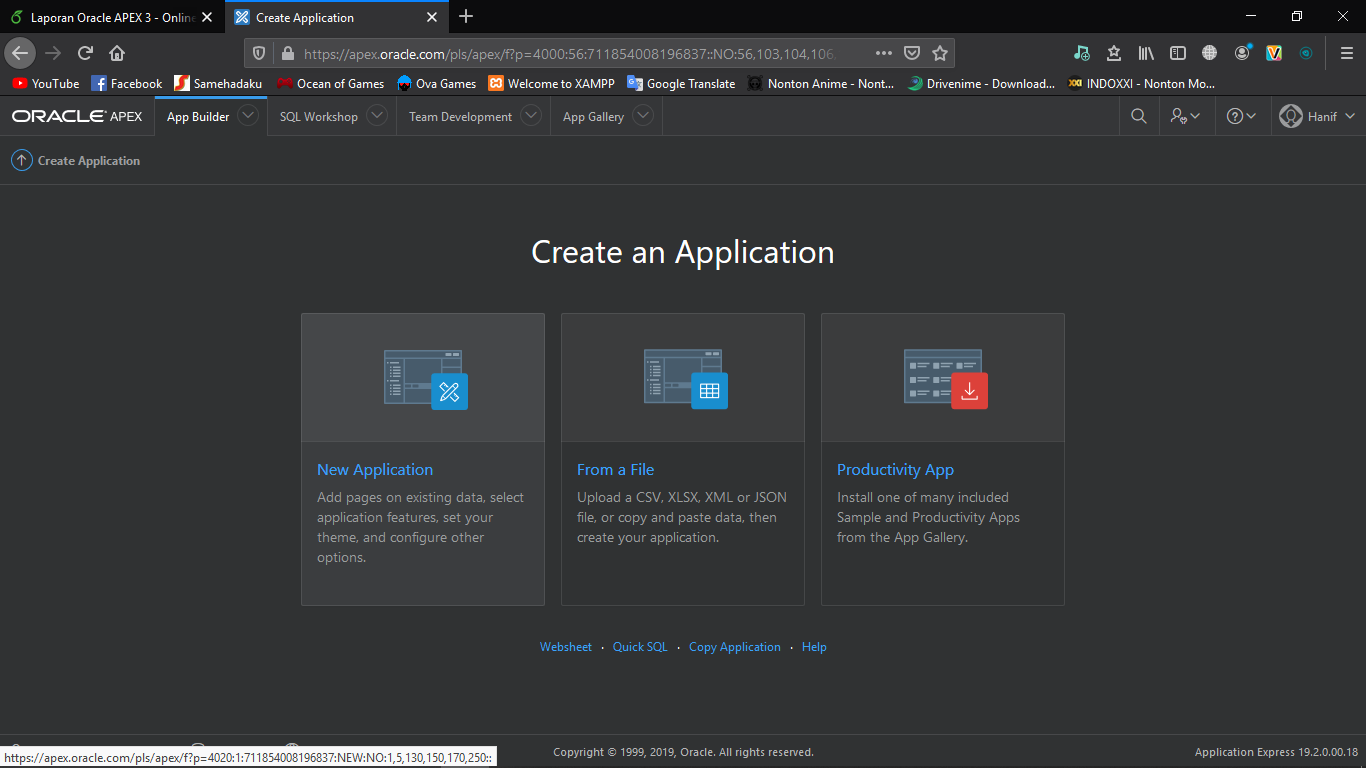
\includegraphics[scale=0.3]{figures/Screenshot(51).png}
    \end{center}
    \end{figure}
    
\begin{figure}[!htbp]
\item[8] Lalu akan muncul tampilan berikut. Masukkan nama aplikasi yaitu Aplikasi Akademik Sederhana dan pilih Master detail.
\begin{center}
    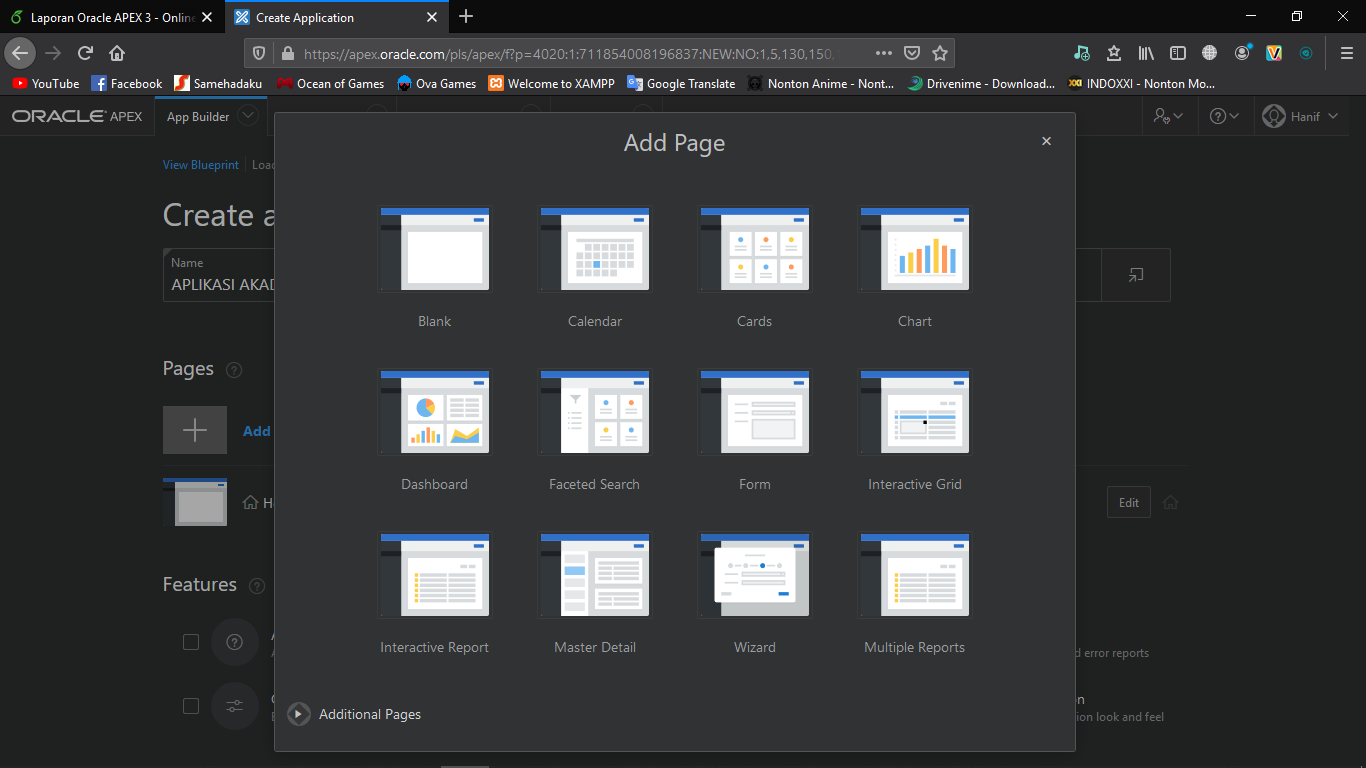
\includegraphics[scale=0.3]{figures/Screenshot(52).png}
    \end{center}
    \end{figure}
    
\begin{figure}[!htbp]
\item[9] Klik add page, pilih model dan pilih tabel. Mausukkan semua tabel yang sudah ada dengan cara yang sama.
\begin{center}
    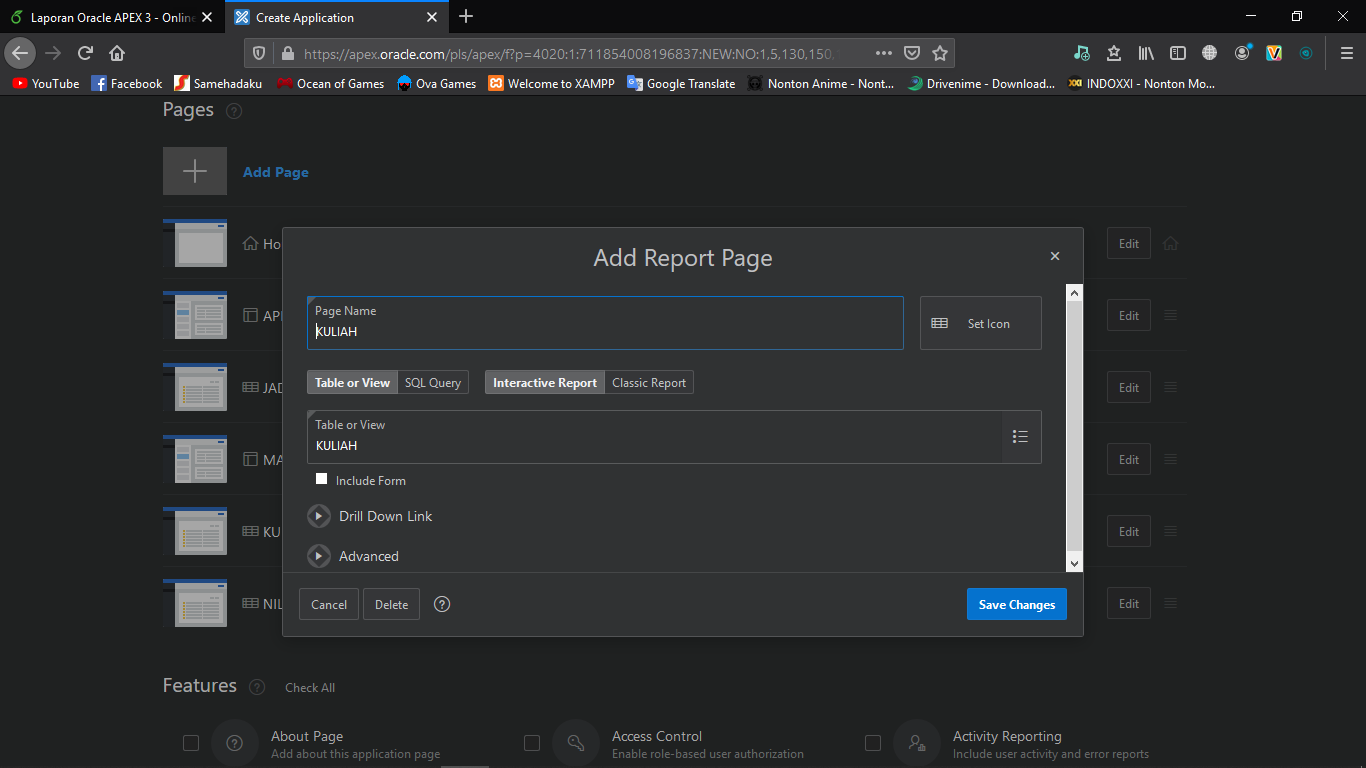
\includegraphics[scale=0.3]{figures/Screenshot(58).png}
    \end{center}
    \end{figure}
    
\begin{figure}[!htbp]
\item[10] Scroll kebawah, klik create application.
\begin{center}
    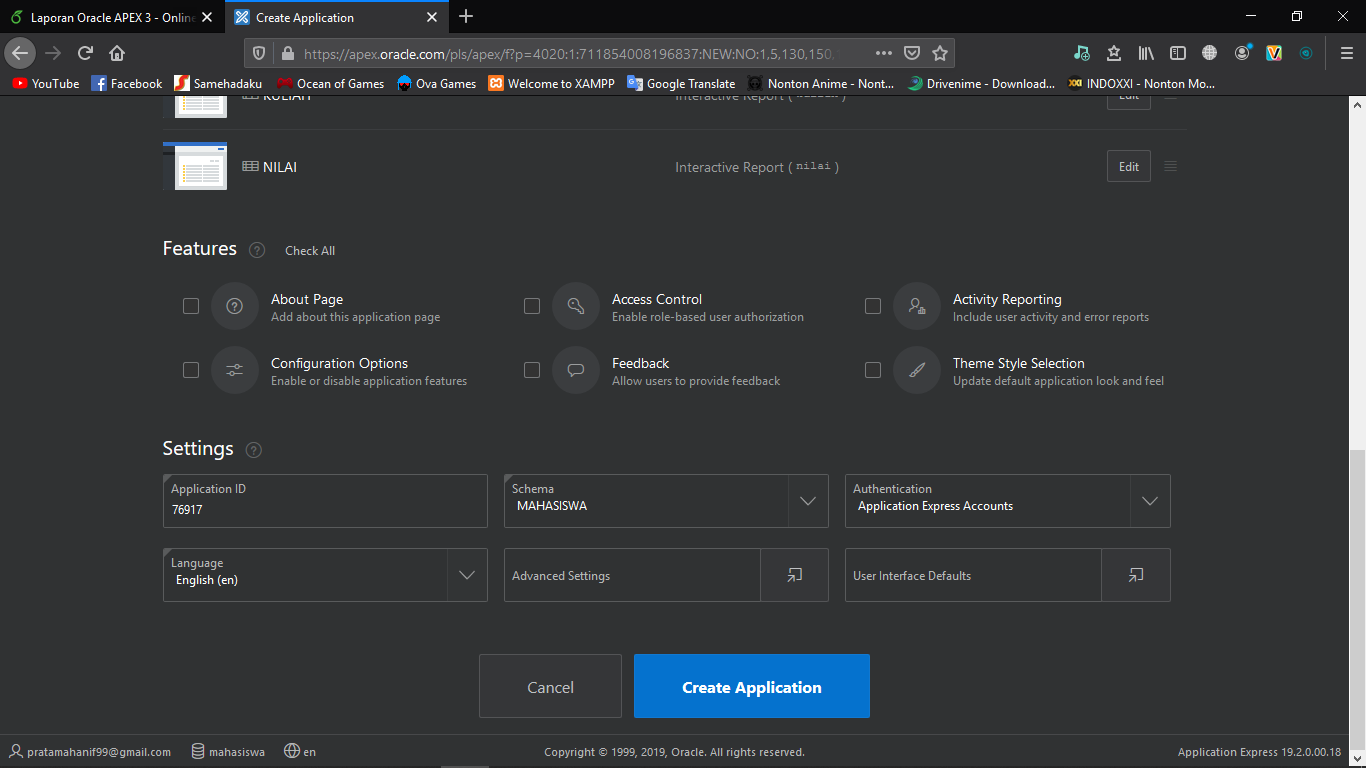
\includegraphics[scale=0.3]{figures/Screenshot(60).png}
    \end{center}
    \end{figure}
    
\begin{figure}[!htbp]
\item[11] Pilih run application.
\begin{center}
    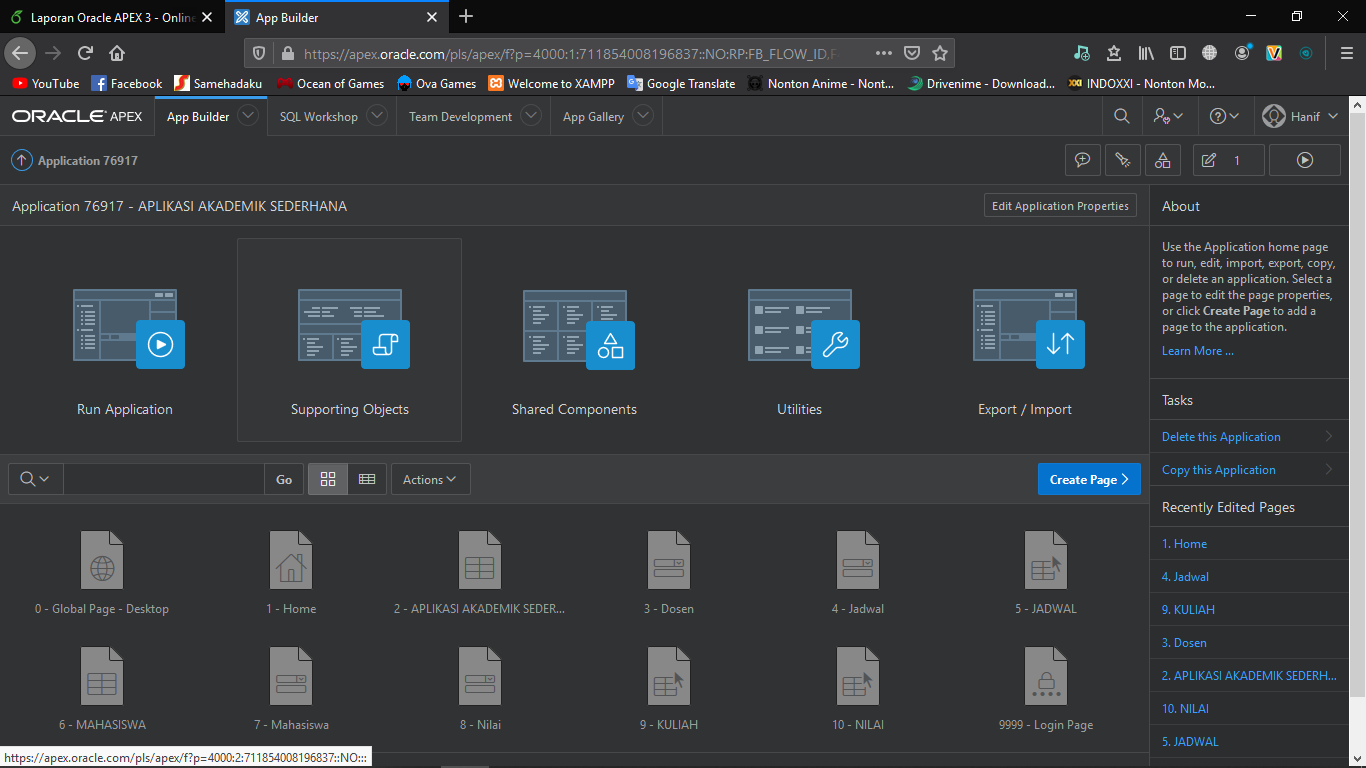
\includegraphics[scale=0.3]{figures/Screenshot(61).png}
    \end{center}
    \end{figure}
    
\begin{figure}[!htbp]
\item[12] Login terlebih dahulu. Masukkan username pratamahanif99@gmail.com dan password Barcalampung\#99 pada URL https://apex.oracle.com/pls/apex/f?p=76917:LOGIN\_DESKTOP:100054287195980:::::
\begin{center}
    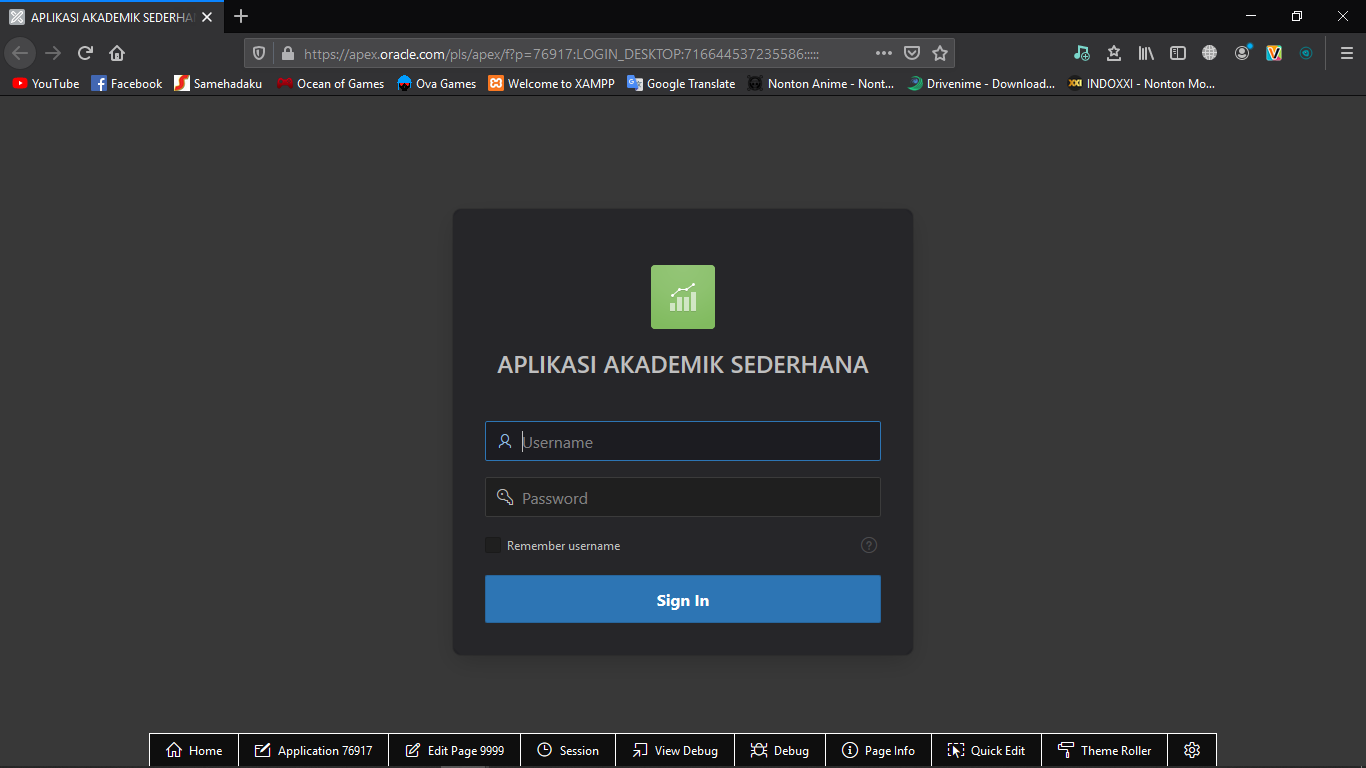
\includegraphics[scale=0.3]{figures/Screenshot(62).png}
    \end{center}
    \end{figure}
    
\begin{figure}[!htbp]
\item[13] Berikut adalah tampilan aplikasi yang sudah dibuat.
\begin{center}
    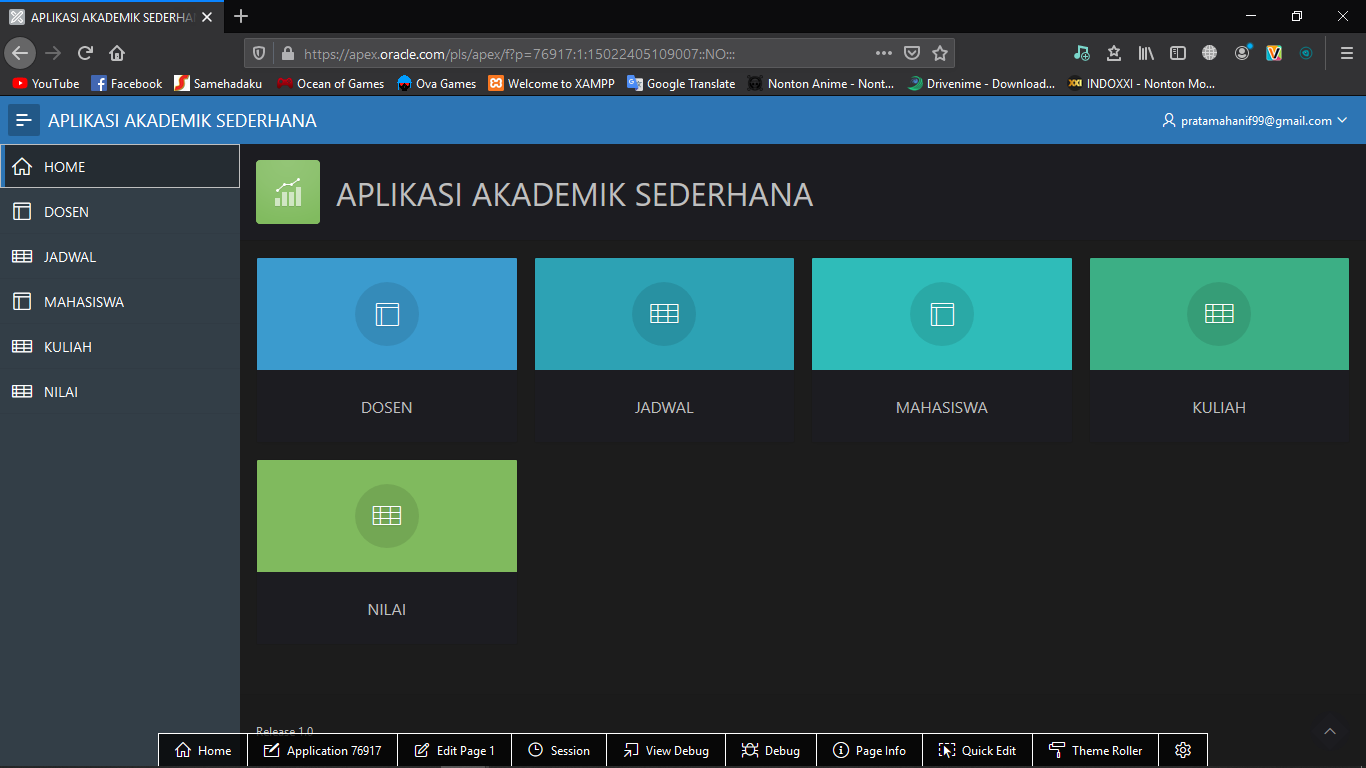
\includegraphics[scale=0.3]{figures/Screenshot(63).png}
    \end{center}
    \end{figure}    
\end{enumerate}


